%\vspace{-0.1in}
\section{Challenges}\label{sec:challenges}

\subsection{Incremental Deployment}\label{sec:incremental}

The protocol stack of the production data center networks copied heavily from the Internet. To the best of our knowledge, all the Cloud Computing providers use Ethernet to construct the physical network and the layer-3 IP protocol for packet forwarding. Furthermore, many, if not all, of the major providers use the well known Internet routing protocols (e.g., BGP, OSPF) for routing and inter-networking.

This is not a coincidence, as the Internet protocol suite and technologies provide the proven scalability and fault-tolerance, and high cost effectiveness due to the economy of scale. 

RoCEv2 is introduced in data center networks to address the performance issues faced by TCP \cite{dcqcn,rdmaatscale} and better support new applications \cite{tensorflow}. RoCEv2 works within the existing network topology (typically Clos based networks) and protocol suite (Ethernet, IP, and UDP). 

In this work, our goal is to make our deadlock prevention design readily deployable without revising existing routing protocols (being distributed or centralized) or introducing new ones. The benefits of incremental deployment is apparent: all the existing services still run without any interruption; all the network configuration, monitoring, management services for the lossy traffic still work as before; and the proven fault-tolerance of the existing routing protocols is extended to the lossless RDMA traffic as well. 

The challenge, however, is that existing routing protocols may cause deadlocks. As we have shown in Figure~\ref{fig:deadlock_example}, deadlocks may happen even when there are no routing loops. Worse, even when a topology may not have deadlocks under normal condition (e.g., a fat-tree without any link failures), deadlocks may happen because of packet reroute due to link or network device failures \cite{shpiner2016unlocking}, which are inevitable in large-scale data centers. 

Our goal is to make our deadlock prevention design work with existing routing protocols. In this paper, we will use the distributed BGP as an example, though our design works for other distributed and centralized routing protocols. 

%Public cloud providers are actively expanding the RoCE deployment using commodity hardware.
%PFC deadlock, though happens occasionally, has been the Sword of Damocles for RoCE networks
%since it causes severe consequence everytime it occurs. We hope to address this problem
%without a disruptively change to the network, so that the solution can be immediately deployed.

%Specifically, we are facing a few practical constraints. First, we do not want to force the network
%operator to change the topology or routing configuration.
%Existing topology and routing configuration has been chosen for various reasons. For example,
%network operators on-purposely implement redundant paths for performance and reliability. However,
%some prior deadlock solutions limit the number of redundant paths, thus are not ideal.

%Second, since most of current datacenter networks do not have a centralized controller that dictates
%each individual flows, the deadlock prevention solution must be decentralized.
%Each switch should perform actions based on local information.
%Finally, we do not change the packet header formats, since commodity switches do not support that.

%We do not claim that these constraints are fundamental. In fact, we are aware that, for example,
%rewiring the topology and designing a special routing protocol may solve the deadlock
%problem. However, we argue that, there exist solutions that do not incur such overhead. In this
%paper, we propose a solution that is the best for incremental deployment.

\subsection{Common IP Routing is Dynamic}\label{sec:reroute}

Keeping existing topology and routing is good for incremental deployment.
Unfortunately, the common network topology and routing, {\em e.g.,} a Clos network~\cite{fat-tree,vl2} with
BGP routing, has the risk of having cyclic buffer dependency, or {\em CBD}.
This is due to the fact that IP routing protocols are by design reactive to the changes in network.

\begin{figure}
	%\vspace{-0.1in}
	\centering
	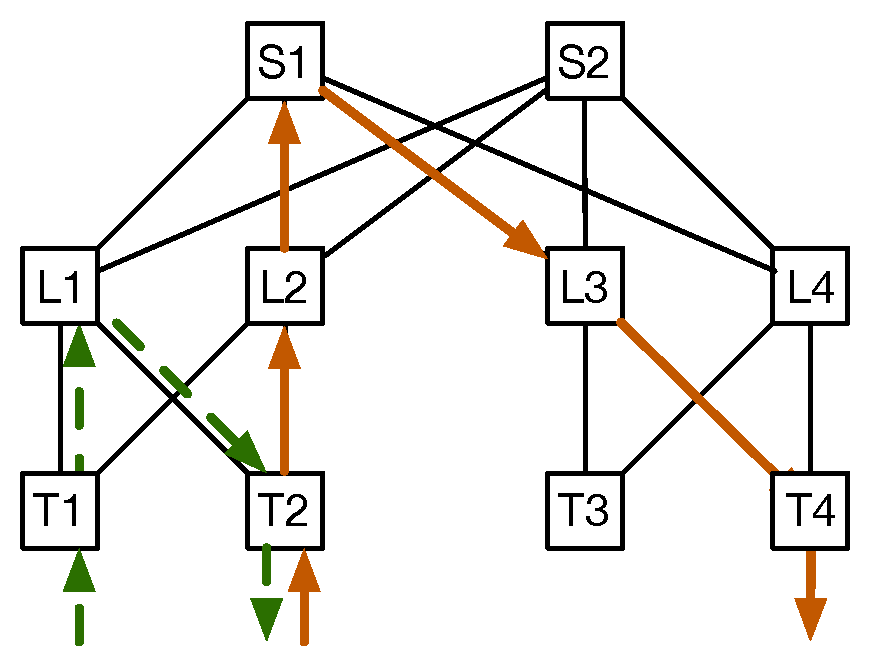
\includegraphics[width=0.4\textwidth] {figs/up-down}
	\caption{UP-DOWN routing in a Clos network.}\label{fig:up-down}
\end{figure}

Take {Figure~\ref{fig:up-down} as an example. If packets always follow the UP-DOWN routing, then deadlock cannot
happen as CBD is not possible. In up-down routing, a packet first goes UP from the source server to one of the common ancestor switches of the source and destination servers, then it goes DOWN from the common ancestor to the destination server.
In UP-DOWN routing, the following property holds: when the packet is on its way UP, it should not go DOWN; when it is on its way DOWN, it should not go UP.

However, packets may deviate from the UP-DOWN paths due to several reasons including link flapping and routing protocol flapping \cite{f10}.
As have shown in \cite{shpiner2016unlocking}, when the UP-DOWN property is broken and packets may reroute multiple times between two layers of switches, and deadlocks may form as a result.

In this paper, we show our measurement results from a large cloud computing provider that UP-DOWN routing property does break in reality and packets can be rerouted with a non negligible probability.

Our measurement works as follows. We instrument the servers to send out IP-in-IP packets to the high-layer switches. The outer source and destination IP addresses are set to the sending server and one of the high layer switches, and the inner source and destination IP addresses are set to the switch and the sending server, respectively. The high-layer switches are configured to decapsulate those IP-in-IP packets that are targeting themselves in hardware.

After decapsulation, the outer IP header is discarded, and the packet is then routed using its inner header. We set a TTL value, 64 in this paper, in the inner IP header. As the packet is forwarded back to the server, the TTL is decremented per hop. For a three-layer Clos network, there are three hops from the highest layer switches to the server. Hence normally the TTL value of the received packets should be 61.

If, however, the TTL value of a received packet is smaller than 61, say 59, we know the received packet was not taking the shortest path, and the packet must have taken a reroute path.

In this paper, for every measurement, a server sends out $n=100$ IP-in-IP probing packets, if the received TTL values are not equal, we know packet reroute happened for this measurement. We then calculate the reroute probability of the measurements as $\frac{M}{N}$, where $M$ is the number of measurements that experienced packet reroute, and $N$ is the total number of measurements. We carried out the measurements for one week in more than 20 data centers. The measurement results are shown in Table~\ref{fig:reroute}.

\begin{table}[t]
\begin{small}
\begin{center}
\begin{tabular}{|r|r|r|c|}
\hline    Date    & Total No.  & Rerouted No.   & Reroute probability \\
\hline 11/01/2016 & 11381533570 & 148416 &  1.3e-5 \\
\hline 11/02/2016 & 11056408780 & 130815 &  1.2e-5 \\
\hline 11/03/2016 & 10316034165 & 104472 &  1.0e-5 \\
\hline 11/04/2016 & 10273000622 & 92555  &  0.9e-5 \\
\hline 11/05/2016 & 10230003382 & 102872 &  1.0e-5 \\
\hline 11/06/2016 & 10491233987 & 106266 &  1.0e-5 \\
\hline 11/07/2016 & 9608289622  & 100916 &  1.1e-5 \\
\hline
\end{tabular}
\end{center}
\caption{Packet reroute measurements in the data centers of a large cloud computing service provider.}\label{fig:reroute}
\end{small}
\end{table}

The most important conclusion we can draw from Table~\ref{fig:reroute} is that packet reroute does happen in data center networks. The reroute probability is around $10^{-5}$. Though $10^{-5}$ is not a big number, given the large traffic volume and the large scale data center networks, the deadlocks due to packet reroute as discussed in \cite{rdmaatscale,shpiner2016unlocking,hu2016deadlocks} do not just exist in paper designs. They are real!

Therefore how to address potential deadlocks due to packet reroute becomes a pressing challenge.

%adding discussions on why packet reroute happen.

\subsection{Limited Number of Lossless Queues}\label{subsec:pfcheadroom}

The number of lossless queues that can be implemented on each switch is limited by two factors. First, the popular ASICs usually support up to eight different classes,
and a few of which must be reserved for lossy traffic. Second, each lossless queue requires certain amount of buffer to operate. This further limits the number of
lossless queues.

In the next we analyze how many lossless priorities we can have based on PFC headroom and buffer space.

A PFC PAUSE frame sent from a receiver to an upstream sender needs some time to arrive and take effect. To avoid packet drops, the receiver must reserve enough buffer to accommodate packets it may receive during this period. The amount of buffer reserved for this purpose is called \textit{PFC headroom}. 

PFC headroom can be calculated by considering the time for a receiver to pause its upstream sender since  PAUSE is triggered. It consists of the following six periods.

\begin{enumerate}
	
\item\textbf{The time to send a PAUSE frame (denoted as $t_{snd}$)}: The transmission of the PAUSE frame  can pass ahead of any other packet queued in the receiver, but cannot preempt another frame currently being transmitted in the same direction. In the worst case, the receiver generates a PAUSE frame right when the first bit of a maximum-size packet has started engaging the transmission logic. So we have  $t_{snd}=(s_{MTU}+s_{PFC})/r_{l}$, where $s_{MTU}$ is the size of a maximum-size packet, $s_{PFC}$ is the size of PFC PAUSE frame and $r_{l}$ is the line rate of network link.

\item\textbf{The time for the PAUSE frame to propagate from the receiver to the sender (denoted as $t_{wire}$)}: The value of  $t_{wire}$ is related to the materia and the length of the network links in use.

\item\textbf{The time to receive a PAUSE frame at the sender (denoted as $t_{rev}$)}: It is easy to know $t_{rev}=s_{PFC}/r_{l}$.

\item\textbf{The time to process a PAUSE frame at the sender (denoted as $t_{pro}$)}:  After a PAUSE frame is received, the sender needs an implementation-dependent amount of time to process it.

\item\textbf{The time to stop packet transmission at the sender (denoted as $t_{stop}$)}: The sender can stop packet transmission only at packet boundaries.  In the worst case, the sender will have completed the process of the PAUSE frame just when the first bit of a maximum-size packet has started engaging the  transmission logic. Hence we have  $t_{snd}=s_{MTU}/r_{l}$.

\item\textbf{The time for the remaining bytes of packets on the link to get drained after packet transmission has stopped (also denoted as $t_{drain}$)}: It is easy to know  $t_{drain}=t_{wire}$.

\end{enumerate}


 To correctly calculate the PFC headroom, we need to further consider the fact that most modern switches divide the switch buffer into cells of fixed size. A buffer cell can only accommodate bytes of a single packet. For example, A 64-byte packet will consume one cell of 100 bytes, and 36 bytes of this cell will remain unused.
 
 We use $s_{cell}$ to denote the size of buffer cell, and $s_{min}$ to denote the minimum size of a packet. In the worst case, the sender sends packets of minimum size in periods 1,2,3,4 and 6, and packets of maximum size in period 5. Hence
 PFC headroom for a single priority per port is (denoted as $b_{hr}$):
 
 
 \begin{eqnarray} \label{eqn:pfcheadroom}
 b_{hr}  & = &  s_{cell}\lceil\frac{(s_{MTU}+2s_{PFC}+2r_{l}t_{wire}+r_{l}t_{pro})}{s_{min}}\rceil \nonumber   \\
 & & +  s_{cell}\lceil\frac{s_{MTU}}{s_{min}}\rceil  
 \end{eqnarray}

For typical TCP/IP based RDMA DCNs, we have $s_{MTU}$ = 1500bytes, $s_{min}$ = 64bytes, $s_{PFC}$ = 64bytes, $t_{wire} \leq$ 1.5us and $t_{pro}\le $ 4us. For Broadcom chipset, we have $s_{cell}$ = 208bytes. According to the above equation, for commodity switches like Arista 7050QX32 which has 32 full duplex 40Gbps ports and 12MB buffer, it requires about 3.8MB buffer to support a single lossless priority. Hence only 2 lossless priorities can be supported.

\textcolor{red}{Discussion: When using 208bytes buffer cell, 100Gbps switches requires 8MB PFC headroom for one lossless priority. This means that only 1 lossless priority can be supported. Do we really need to consider the constraint of buffer cell? This sounds like an engineer issue, and can be fixed by using a smaller buffer cell.}

%\textbf{Reducing the PFC headroom}: For tree-based topologies like Fat-tree, packets of consecutive priority classes will not enter the same switch. So the number of priority classes a switch needs to support is halved.  This reduces the needed PFC headroom to $2816$KB, which is about $22.9\%$ of the total 12MB switch buffer.


%For typical TCP/IP based RDMA DCNs, we have $s_{MTU}=1500$bytes, $s_{PFC}=64$bytes. The length of links used in a single DCN is usually no larger than 300 meters~\cite{rdmaatscale}. As every 100 meters of link delays the reception of a packet by about 500ns for copper cables~\cite{pfcheadroom}, we have $t_{wire} \leq 1.5us$.
%
%The value of  $t_{pro}$ is implementation related. Let a quanta be the time needed to transmit 512 bits at the current network speed. The PFC definition caps this time to 60 quanta for any implementation~\cite{pfcheadroom}. Hence we have $r_l*t_{pro}=512 * 60 = 30,720 $ bits.
%
%According to the above parameters, when  $r_l=40Gbps$, the per port per priority PFC headroom $b_{hr} \leq 21968$ bytes $\approx 22$ KB.
%
%\textbf{PFC headroom of a switch:} For a $n$ port switch which supports $k$ priority classes, PFC PAUSE is possible to be triggered at all ports and priority classes simultaneously. So we should at least reserve $n*k*b_{hr}$ buffers as PFC headroom at every switch.
%
%For commodity switches like Arista 7050QX32 which has 32 full duplex 40Gbps ports, when supporting 8 priority classes, it requires about $32*8*22=5632$KB buffer as the PFC headroom.

%Let $b_{rev}$ be the maximum bytes of packets the receiver can receive during the above 6 periods. We have:
%
%
%\begin{eqnarray} \label{eqn:pfcheadroom}
%b_{rev} &=& r_{l}*(t_{snd}+t_{wire}+t_{rev}+t_{pro}+t_{stop}+t_{drain})     \nonumber \\
%&=& 2(s_{MTU}+s_{PFC}+r_l*t_{wire})+r_l*t_{pro}
%\end{eqnarray}

%\subsection{Necessary Buffer for Achieving Work-Conservation}\label{subsec:bufferthroughput}
%
%According to the rule-of-thumb~\cite{crtt,sizingrouterbuffer}, we at least need a buffer of size $b = C*RTT$ per port for achieving work-conservation, where RTT is the average round-trip time, and C is the link capacity. As our TTL-based solution allocates dedicated buffer to different priority classes, for a switch of n ports, when supporting $k$ priority classes, it demands a buffer of size $n*k*C*RTT$.
%
%Assuming that the average RTT in the DCN is $50$us. For Arista 7050QX32 switch, when supporting 8 priority classes, we need to reserve a buffer of size $32*8*40Gbps*50us=64MB$. This apparently exceeds the total buffer size of most commodity switches. The key to solving this problem is to let packets of different priority classes share some buffer.
%
%On the other hand, we also need to ensure that PFC threshold is not reached before the switch has a chance to mark packets with ECN. This has been well discussed in DCQCN~\cite{dcqcn}. Basically, we can leverage a dynamic PFC thresholding scheme to dynamically share the switch buffer among different ports.

%\textbf{Reducing the necessary buffer for achieving work-conservation}: The main problem here is that our TTL-based solution allocates dedicated buffer to different priority classes. To solve this problem, instead of simply allocating dedicated buffer to different priority classes, we can let packets of different priority classes to have both dedicated and shared buffer.
%
%Specifically, we divide the switch buffer into $k+1$ partitions. The first $k$ partitions are dedicated for the k priority classes, correspondingly. The $k+1$ partition is shared by all the priority classes. If a packet is classified as priority class $i$, at first the switch will check whether partion $i$ has enough spare buffer to accommodate this packet. If yes, this packet will be placed in partition $i$. Otherwise, the switch will place this packet in partition $k+1$.
%
%The original dynamic PFC thresholding scheme cannot be directly applied under the new buffer allocation scheme. Hence we modify it as follows. Let $b_i$ be the size of partition $i$, $t^i_{PFC}$ be the PFC threshold for priority class $i$, $s_i$ be the amount of buffer of partition $i$ that is currently occupied. We have
%
%\begin{eqnarray} \label{eqn:pfcthreshold}
%t^i_{PFC} &=& \alpha\frac{b_i}{\sum_{j=1}^k b_j} (b_{k+1}-s_{k+1}) + \alpha (b_i-s_i)
%\end{eqnarray}
%
%The intuition behind Equation~\ref{eqn:pfcthreshold} is to share the buffer of partition $k+1$ among different priority classes with respect to the weight $\frac{b_i}{\sum_{j=1}^k b_j}$. As for the buffer of dedicated partitions, we follow the idea of original dynamic PFC thresholding scheme to dynamically share it among different ports within the same priority class.
%
%Under the new buffer allocation scheme and the new dynamic PFC thresholding scheme, the buffer needed for achieving work-conservation is reduced to
%$n*C*RTT$, which is within the buffer capacity of most commodity switches.
%\textbf{ Case of multiple priority classes:} When $k$ priority classes are enabled simultaneously at a single port, we cannot simply calculate the PFC headroom of a switch as $k*b_{hr}$. The reason is that in this case packets of any priority class cannot be transmitted at full line rate as the bandwidth is now shared by $k$ priority classes. Let $r_i$ be the packet transmission rate of priority class $i$, $1\leq i \leq k$. The per port PFC headroom of priority class $i$ can be expressed using the following equation
%
%\begin{eqnarray} \label{eqn:mpriority}
%b^i_{hr} &=& r_{i}*(t_{snd}+t_{wire}+t_{rev}+t_{pro}+t_{stop}+t_{wire})     \nonumber \\
%&=& 2(s_{MTU}+s_{PFC}+r_i*t_{wire})+r_i*t_{pro}
%\end{eqnarray}
%
%Then the total per port PFC headroom of all the $k$ priority classes can be calculated as
%
%\begin{eqnarray} \label{eqn:sumpriority}
%b_{hr}&=&\sum\limits_{i=1}^k b^i_{hr}       \nonumber \\
%&=& 2k(s_{MTU}+s_{PFC})+ 2\sum\limits_{i=1}^k r_i*t_{wire}+\sum\limits_{i=1}^kr_i*t_{pro}     \nonumber \\
%&=& 2k(s_{MTU}+s_{PFC})+ 2r_l*t_{wire}+r_l*t_{pro}
%\end{eqnarray}
